\documentclass[landscape]{progbookcn}
\usepackage{lmodern}
\usepackage{multicol}

\newcommand{\bigo}[1]{$\mathcal{O}$(#1)}

\DeclareMathSymbol{\mlq}{\mathord}{operators}{``}
\DeclareMathSymbol{\mrq}{\mathord}{operators}{`'}

\begin{document}

%% title page
    \begin{titlepage}
    \vspace*{25ex}
  
    \hspace{0.05\textwidth}\begin{minipage}{.9\textwidth}
      \flushright
  
      %%中文书名
      {\zihao{1}\textbf{算法学习:AcWing}}
  
      \rule{\linewidth}{.5pt}
  
      \vspace{2ex}
  
      %% 英文书名
      {\zihao{2}\textsf{Algorithm Learning: AcWing}} \\
  
      \vspace{20ex}
  
      %% 作者
      {\zihao{4}\textit{吴小强}~编著}
    \end{minipage}
  
    \vfill
  
    \centering
    {\zihao{4}深圳 ~$\bullet$ ~SHENZHEN}
  \end{titlepage}
    \thispagestyle{empty}

    \frontmatter

    \chapter{前言}

% 本书是在 \href{https://www.acwing.com/}{AcWing} 学习的记录,序言留待后续补足。

%% 目录
    \clearpage
    {
        \hypersetup{hidelinks}
        \tableofcontents
    }

    \mainmatter


    \part{算法基础}
    \label{alg_foundation_part}
    \chapter{算法基础}

\section{快速排序}
\subsection{AcWing 785. 快速排序}

\begin{titledbox}{AcWing 785. 快速排序}
  给定你一个长度为 $n$ 的整数数列。请你使用快速排序对这个数列按照从小到大进行排序。并将排好序的数列按顺序输出。

  输入格式:

  输入共两行,第一行包含整数 $n$。第二行包含 $n$ 个整数(所有整数均在 $1 \sim 10^9$ 范围内),表示整个数列。

  输出格式:

  输出共一行,包含 $n$ 个整数,表示排好序的数列。

  数据范围:$1 \le n \le 100000$

  输入样例:

  5

  3 1 2 4 5

  输出样例:

  1 2 3 4 5
\end{titledbox}

快速排序算法基于\textbf{分治}算法,以一个数来作为分治的节点。

随机选取数组中的某个元素$x$作为分界点,操作数组中的元素使得数组被分割为两个部分,左边一侧的元素小于等于$x$,右边一侧则大于等于$x$。接下来递归的对左右两侧数组进行操作,直到最小数组只有一个元素则完成排序。

主要步骤如下:
\begin{enumerate}
  \item 确定分界点$x$,可取值:\lstinline{q[l]}, \lstinline{q[r]}, \lstinline{q[(l + r) >> 1]}, random value
  \item 调整数组,使得左边小于等于$x$,右边大于等于$x$
  \item 递归处理左右两段
\end{enumerate}

\begin{mycpptwocol}[quick sort]
#include <stdio.h>
#include <stdlib.h>

void swap(int *q, int a, int b) {
    int tmp = q[a];
    q[a] = q[b];
    q[b] = tmp;
}

void quick_sort(int *q, int l, int r)
{
    if (l >= r) {
        return;
    }
    int x = q[(l + r) >> 1];
    int i = l - 1;
    int j = r + 1;
    while (i < j) {
        do i++; while (q[i] < x);
        do j--; while (q[j] > x);
        if (i < j) {
            swap(q, i, j);
        }
    }
    quick_sort(q, l, j);
    quick_sort(q, j + 1, r);
}

int main() {
    int n;
    scanf("%d", &n);
    int *q = (int *)calloc(sizeof(int), n);
    if (q == NULL) {
        return -1;
    }
    for (int i = 0; i < n; i++) {
        scanf("%d", q + i);
    }

    quick_sort(q, 0, n - 1);

    for (int i = 0; i < n; i++) {
        printf("%d ", q[i]);
    } 
    free(q);
    return 0;
}
\end{mycpptwocol}

从上述代码段中可以清晰看到递归处理的过程,每次选取分界点,之后将左右两侧的元素进行调整,此处采用双指针算法。

\begin{keypoint}
    这里有两个问题:
    \begin{enumerate}
        \item 在选择x时选择\lstinline{q[l]}则在递归是不能选用\lstinline{i},会出现边界问题 | \lstinline{i - 1, i}
        \item 在选择x时选择\lstinline{q[r]}则在递归是不能选用\lstinline{j},会出现边界问题 | \lstinline{j, j + 1}
    \end{enumerate}

    边界用例可使用\lstinline{1, 2}这个例子,会有递归不结束的问题
\end{keypoint}

\begin{information}
  该算法\textbf{不稳定},因为\lstinline{q[i]}和\lstinline{q[j]}相等的时候会发生交换。

  这里调整数组的部分是难点,怎么优雅的调整数组?暴力做法可以开辟两个辅助数组来存储。双指针做法优雅简洁。
\end{information}

时间复杂度分析:

\subsection{AcWing 786. 第k个数}
快速选择算法可选出有序数组中的第$k$个数,与快排中逻辑相同,左侧的元素都小于$x$右侧元素都大于$x$。如果左侧元素的数量大于等于$k$则表示第$k$个元素在左侧数组中,反之则在右侧数组中寻找$k-\text{left length}$的元素。

\begin{titledbox}{AcWing 786. 第k个数}
给定一个长度为 $n$ 的整数数列,以及一个整数 $k$,请用快速选择算法求出数列从小到大排序后的第 $k$ 个数。

输入格式:

第一行包含两个整数 $n$ 和 $k$。
第二行包含 $n$ 个整数(所有整数均在 $1 \sim 10^9$ 范围内),表示整数数列。

输出格式:

输出一个整数,表示数列的第 $k$ 小数。

数据范围:

$1 \le n \le 100000$,
$1 \le k \le n$

输入样例:

5 3

2 4 1 5 3


输出样例:

3
\end{titledbox}


\begin{mycpptwocol}[find kth smallest number]
#include <stdio.h>
#include <stdlib.h>

int q_select(int *q, int l,
             int r, int k) {
    if (r <= l) {
        return q[l];
    }

    int x = q[(l + r) >> 1];
    int i = l - 1;
    int j = r + 1;

    while (i < j) {
        do i++; while(q[i] < x);
        do j--; while(q[j] > x);

        if (i < j) {
            int tmp = q[i];
            q[i] = q[j];
            q[j] = tmp;
        }
    }

    int length = j - l + 1;
    if (length < k) {
        return q_select(q, j + 1, r,
            k - length);
    } else {
        return q_select(q, l, j, k);
    }
}

int main()
{
    int n;
    int k;
    scanf("%d %d", &n, &k);
    int *q = (int *)calloc(sizeof(int), n);
    if (q == NULL) {
        return -1;
    }
    for (int i = 0; i < n; i++) {
        scanf("%d", q + i);
    }
    int ret = q_select(q, 0, n - 1, k);
    printf("%d", ret);
    return 0;
}
\end{mycpptwocol}

\section{归并排序}
归并排序同样是基于\textbf{分治}算法,不过是以整个数组的中间位置来分。

将数组分割成两个已经分别排序好的有序数组,再将其二者合并即可。此方法需要有单独的空间来存放合并的临时结果,再将临时结果写入到原始区域中。

主要步骤如下:
\begin{enumerate}
  \item 确定分界点,\lstinline{mid = (l + r) >> 1}
  \item 递归排序左右两边
  \item 归并,将两个有序的子数组合二为一
\end{enumerate}

\subsection{AcWing 787. 归并排序}
\begin{titledbox}{AcWing 787. 归并排序}
    给定你一个长度为 $n$ 的整数数列。请你使用归并排序对这个数列按照从小到大进行排序。并将排好序的数列按顺序输出。
  
    输入格式:
  
    输入共两行,第一行包含整数 $n$。第二行包含 $n$ 个整数(所有整数均在 $1 \sim 10^9$ 范围内),表示整个数列。
  
    输出格式:
  
    输出共一行,包含 $n$ 个整数,表示排好序的数列。
  
    数据范围:$1 \le n \le 100000$
  
    输入样例:
  
    5
  
    3 1 2 4 5
  
    输出样例:
  
    1 2 3 4 5
\end{titledbox}

\begin{mycpptwocol}[merge sort]
#include <stdio.h>
#include <stdlib.h>

#define N 100010

int backup[N];

void merge_sort(int *q, int l, int r)
{
    if (r <= l) {
        return;
    }
    int mid = (l + r) >> 1;
    merge_sort(q, l, mid);
    merge_sort(q, mid + 1, r);
    int k = 0;
    int i = l;
    int j = mid + 1;
    while (i <= mid && j <= r) {
        if (q[i] <= q[j]) {
            backup[k++] = q[i++];
        }
        if (q[j] < q[i]) {
            backup[k++] = q[j++];
        }
    }
    while (i <= mid) {
        backup[k++] = q[i++];
    }
    while (j <= r) {
        backup[k++] = q[j++];
    }
    
    for (i = l, j = 0; j < k; i++, j++) {
        q[i] = backup[j];
    }
}

int main()
{
    int n;
    scanf("%d", &n);
    int *q = (int *)calloc(sizeof(int), n);
    if (q == NULL) {
        return -1;
    }
    for (int i = 0; i < n; i++) {
        scanf("%d", q + i);
    }
    merge_sort(q, 0, n - 1);
    for (int i = 0; i < n; i++) {
        printf("%d ", q[i]);
    }
    return 0;
}
\end{mycpptwocol}

双指针算法做归并

\begin{keypoint}
    这里归并两个子数组之后要写回去,\lstinline{backup}数组只是临时存储使用。
\end{keypoint}

\subsection{AcWing 788. 逆序对的数量}
\begin{titledbox}{AcWing 788. 逆序对的数量}
    给定一个长度为 $n$ 的整数数列,请你计算数列中的逆序对的数量。
    逆序对的定义如下:对于数列的第 $i$ 个和第 $j$ 个元素,如果满足 $i < j$ 且 $a[i] > a[j]$,则其为一个逆序对;否则不是。
    
    输入格式:

    第一行包含整数 $n$,表示数列的长度。第二行包含 $n$ 个整数,表示整个数列。
    
    输出格式:
    
    输出一个整数,表示逆序对的个数。

    数据范围

    $1 \le n \le 100000$,
    数列中的元素的取值范围 $[1,10^9]$。
    
    输入样例:

    2 3 4 5 6 1
    
    输出样例:
    
    5
\end{titledbox}

分治思路,将整个区间一分为二。考虑到归并排序的时候需要将两个有序数组合并,此时恰好可以做逆序对的统计。假设有一种算法,可以将数组排序的过程中统计该数组中的逆序对数量,则问题变为怎么统计两个有序数组中合起来的逆序对。

\begin{mycpptwocol}[归并排序计算逆序对数量]
#include <stdio.h>
#include <stdlib.h>

long long merge_sort(int *q, int *tmp,
                     int l, int r) {
    if (l >= r) {
        return 0;
    }
    int mid = (l + r) >> 1;
    // 左侧的数组已统计逆序对且已经排序,右侧同样
    long long res = merge_sort(q, tmp, l, mid) + merge_sort(q, tmp, mid + 1, r);
    // 统计两个有序数组合起来的逆序对
    int i = l;
    int j = mid + 1;
    int k = 0;
    while (i <= mid && j <= r) {
        if (q[i] > q[j]) {
            res += mid - i + 1;
            tmp[k++] = q[j++];
        } else {
            tmp[k++] = q[i++];
        }
    }
    
    while (i <= mid) {
        tmp[k++] = q[i++];
    }
    while (j <= r) {
        tmp[k++] = q[j++];
    }
    for (i = l, j = 0; i <= r;
         i++, j++) {
        q[i] = tmp[j];
    }
    
    return res;
}

int main()
{
    int n;
    scanf("%d", &n);
    int *q = (int *)calloc(n, sizeof(int));
    if (q == NULL) {
        return -1;
    }
    int *tmp = (int *)calloc(n, sizeof(int));
    if (tmp == NULL) {
        free(q);
        return -1;
    }
    for(int i = 0; i < n; i++) {
        scanf("%d", &q[i]);
    }
    
    printf("%ld", merge_sort(q, tmp, 0, n - 1));

    return 0;
}
\end{mycpptwocol}
\section{二分}
整数二分和浮点数二分,二分即查找一个边界值,在左侧满足某种性质,右侧不满足。

二分用模版如下:
\begin{mycpptwocol}[二分模版]
// 区间[l, r]被划分为[l, mid] 和
// [mid + 1, r]时使用, 往左找
int bsearch_1(int l, int r)
{
    while (l < r) {
        mid = (l + r) / 2;
        if (Check(mid)) {
            r = mid;
        } else {
            l = mid + 1;
        }
    }
}
// 区间[l, r]被划分为[l, mid - 1] 和
// [mid, r]时使用,往右找
int bsearch_2(int l, int r)
{
    while (l < r) {
        mid = (l + r + 1) / 2;
        if (Check(mid)) {
            l = mid;
        } else {
            r = mid - 1;
        }
    }
}
\end{mycpptwocol}

\begin{keypoint}
    每次要保证答案在区间中。

    第二个模版加一的原因在于,如果某次循环结束后,\lstinline{l = r - 1},如果不加1,此时因为向下取整的缘故\lstinline{mid = l},check成功后\lstinline{l}被再次赋值为\lstinline{mid}即\lstinline{l},则此时进入死循环。
\end{keypoint}

\subsection{AcWing 789. 数的范围}
\begin{titledbox}{AcWing 789. 数的范围}
给定一个按照升序排列的长度为 $n$ 的整数数组,以及 $q$ 个查询。对于每个查询,返回一个元素 $k$ 的起始位置和终止位置(位置从 $0$ 开始计数)。如果数组中不存在该元素,则返回\lstinline{-1 -1}。

输入格式:

第一行包含整数 $n$ 和 $q$,表示数组长度和询问个数。第二行包含 $n$ 个整数(均在 $1 \sim 10000$ 范围内),表示完整数组。接下来 $q$ 行,每行包含一个整数 $k$,表示一个询问元素。

输出格式:

共 $q$ 行,每行包含两个整数,表示所求元素的起始位置和终止位置。

数据范围
$1 \le n \le 100000$,
$1 \le q \le 10000$,
$1 \le k \le 10000$

输入样例:

6 3

1 2 2 3 3 4

3

4

5

输出样例:

3 4

5 5

-1 -1
\end{titledbox}


\begin{mycpptwocol}[binary search]
#include <stdio.h>
#include <stdlib.h>

int b_search_l(int *q, int l,
               int r, int t) {
    while (l < r) {
        int mid = (l + r) >> 1;
        if (q[mid] >= t) {
            r = mid;
        } else {
            l = mid + 1;
        }
    }
    if (q[l] != t) {
        return -1;
    }
    return l;
}

int b_search_r(int *q, int l,
               int r, int t) {
    while (l < r) {
        int mid = (l + r) / 2 + 1;
        if (q[mid] <= t) {
            l = mid;
        } else {
            r = mid - 1;
        }
    }
    if (q[l] != t) {
        return -1;
    }
    return l;
}

int main()
{
    int n;
    int q;
    scanf("%d %d", &n, &q);
    int *q = (int *)calloc(sizeof(int), n);
    if (q == NULL) {
        return -1;
    }
    for (int i = 0; i < n; i++) {
        scanf("%d", q + i);
    }
    while(q--) {
        int t;
        scanf("%d", &t);
        printf("%d %d\n",
        b_search_l(q, 0, n - 1, t),
        b_search_r(q, 0, n - 1, t));
    }
    return 0;
}
\end{mycpptwocol}

\begin{exclamation}
    这里不能使用\lstinline{bsearch}函数来完成左端点的搜索,因为该函数在面对重复值时返回值不确定,是未定义行为。
\end{exclamation}

\subsection{AcWing 790. 数的三次方根}
\begin{titledbox}{AcWing 790. 数的三次方根}
    给定一个浮点数 $n$,求它的三次方根。

    输入格式:

    共一行,包含一个浮点数 $n$。

    输出格式:

    共一行,包含一个浮点数,表示问题的解。
    
    注意,结果保留 $6$ 位小数。
    
    数据范围:

    $-10000 \le n \le 10000$
    
    输入样例:
    
    1000.00
    
    输出样例:

    10.000000
\end{titledbox}
\section{高精度}

\section{前缀和与差分}
\begin{enumerate}
    \item 前缀和可方便地求取数组中某个区间的元素和,或者矩阵的子矩阵的和 O(1)
    \item 差分和方便的将数组某个区间的所有元素加上一个数,O(1)时间复杂度
\end{enumerate}

\section{双指针算法}


\section{位运算}


\section{离散化}


\section{区间合并}
    \chapter{数据结构}
    \chapter{搜索和图论}

用树来展示DFS和BFS的区别如下,其中 $h$ 表示树的深度。可见,DFS在空间上具有更大的优势,而BFS则为指数级别。
\begin{table}[!ht]
    \centering
    \begin{tabular}{|c|c|c|l|}
        \hline
        ~   & 数据结构  & 空间           & ~                        \\ \hline
        DFS & stack & \bigo{$h$}   & 不具有最短性                   \\ \hline
        BFS & queue & \bigo{$2^h$} & 第一次扩展到最近点,最短路性质(边的权重为1时) \\ \hline
    \end{tabular}
\end{table}
可见,因为BFS的最短路性质,当需要解决最小操作数、最短距离、最短路等问题时,可以尝试使用BFS。而当题目难以思考时,可尝试DFS。

稠密图:邻接矩阵 \inlinecode{g[N][N]}, a和b之间是否有边,且边的权重是多少

稀疏图:邻接表 \inlinecode{h[N], e[N], ne[N], idx}, 和拉链法的哈希是一样的数据结构


\section{DFS}
从搜索树的角度来看,每一个DFS都对应一个搜索树。DFS最重要的是考虑搜索顺序,以什么顺序进行解空间的遍历。

回溯:回溯的过程由递归处理,每次需要手动维护自己的数据结构,保证恢复现场。

剪枝:

\subsection{AcWing 842. 排列数字}
\begin{titledbox}{AcWing 842. 排列数字}
    给定一个整数 $n$,将数字 $1 \sim n$ 排成一排,将会有很多种排列方法。现在,请你按照字典序将所有的排列方法输出。

    输入格式:

    共一行,包含一个整数 $n$。

    输出格式:

    按字典序输出所有排列方案,每个方案占一行。

    数据范围:

    $1 \le n \le 7$

    \begin{inputblock}
        3
    \end{inputblock}
    \begin{outputblock}
        1 2 3 \\
        1 3 2 \\
        2 1 3 \\
        2 3 1 \\
        3 1 2 \\
        3 2 1
    \end{outputblock}
\end{titledbox}

\begin{mycpptwocol}[排列数字]
    #include <stdio.h>
    #include <stdbool.h>

    #define N 10

    int path[N];
    bool st[N];

    void dfs(int u, int n) {
        if (u == n) {
            for (int i = 0; i < n; i++) {
                printf("%d ", path[i]);
            }
            printf("\n");
            return;
        }
        for (int i = 1; i <= n; i++) {
            if (!st[i]) {
                path[u] = i;
                st[i] = true;
                dfs(u + 1, n);
                st[i] = false;
            }
        }
    }

    int main() {
        int n;
        scanf("%d", &n);
        dfs(0, n);
        return 0;
    }
\end{mycpptwocol}

\subsection{AcWing 843. n-皇后问题}
\begin{titledbox}{AcWing 843. n-皇后问题}
    $n-$皇后问题是指将 $n$ 个皇后放在 $n \times n$ 的国际象棋棋盘上,使得皇后不能相互攻击到,即任意两个皇后都不能处于同一行、同一列或同一斜线上。

    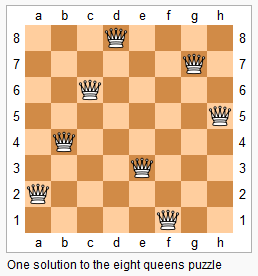
\includegraphics[width=0.3\textwidth]{n-queen.png}

    现在给定整数 $n$,请你输出所有的满足条件的棋子摆法。

    输入格式:

    共一行,包含整数 $n$。

    输出格式:

    每个解决方案占 $n$ 行,每行输出一个长度为 $n$ 的字符串,用来表示完整的棋盘状态。
    其中 \inlinecode{.} 表示某一个位置的方格状态为空,\inlinecode{Q} 表示某一个位置的方格上摆着皇后。每个方案输出完成后,输出一个空行。\textbf{注意:行末不能有多余空格。}输出方案的顺序任意,只要不重复且没有遗漏即可。

    数据范围:

    $1 \le n \le 9$

    \begin{inputblock}
        4
    \end{inputblock}
    \begin{outputblock}
        .Q.. \\
        ...Q \\
        Q... \\
        ..Q. \\

        ..Q. \\
        Q... \\
        ...Q \\
        .Q..
    \end{outputblock}
\end{titledbox}

有两种解法,第一种:因发现每一行每一列有且仅有一个皇后,可以枚举每一行,来看看可以将皇后放置在第几列。

\begin{mycpptwocol}[n-皇后问题:解法一]
    #include <stdio.h>
    #include <stdlib.h>
    #include <string.h>
    #include <stdbool.h>

    #define N 20

    char g[N][N];
    bool col[N];
    bool dg[N];
    bool udg[N];

    void dfs(int u, int n) {
        if (u == n) {
            for (int i = 0; i < n; i++) {
                puts(g[i]);
            }
            printf("\n");
            return;
        }
        for (int i = 0; i < n; i++) {
            if (col[i] || dg[u + i] || udg[u - i + n]) {
                continue;
            }
            g[u][i] = 'Q';
            col[i] = dg[u + i] = udg[u - i + n] = true;
            dfs(u + 1, n);
            g[u][i] = '.';
            col[i] = dg[u + i] = udg[u - i + n] = false;
        }
    }

    int main() {
        int n;
        scanf("%d", &n);
        for (int i = 0; i < n; i++) {
            for (int j = 0; j < n; j++) {
                g[i][j] = '.';
            }
        }
        dfs(0,  n);
        return 0;
    }
\end{mycpptwocol}

解法二:从左上角开始枚举每一个格子,每个格子有两种状态(放或者不放),在枚举过程中检查每一个格子是否可以继续放置。若皇后数量已经达到最大数量则找到了一个方案

\begin{mycpptwocol}[n-皇后问题:解法二]
    #include <stdio.h>
    #include <stdlib.h>
    #include <string.h>
    #include <stdbool.h>

    #define N 20

    char g[N][N];
    bool row[N];
    bool col[N];
    bool dg[N];
    bool udg[N];

    void dfs(int x, int y, int s, int n) {
        if (y == n) {
            y = 0;
            x++;
        }
        if (x == n) {
            if (s == n) {
                for (int i = 0; i < n; i++) {
                    puts(g[i]);
                }
                puts("");
            }
            return;
        }
        // do not put queen here
        dfs(x, y + 1, s, n);

        // put queen here
        if (!row[x] && !col[y] && !dg[x + y] && !udg[x - y + n]) {
            g[x][y] = 'Q';
            row[x] = col[y] = dg[x + y] = udg[x - y + n] = true;
            dfs(x, y + 1, s + 1, n);
            g[x][y] = '.';
            row[x] = col[y] = dg[x + y] = udg[x - y + n] = false;
        }
    }

    int main() {
        int n;
        scanf("%d", &n);
        for (int i = 0; i < n; i++) {
            for (int j = 0; j < n; j++) {
                g[i][j] = '.';
            }
        }
        dfs(0, 0, 0, n);
        return 0;
    }
\end{mycpptwocol}


\section{BFS}

宽度优先搜索的基本思路是初始化一个队列,需要决定队列中存储的是什么。进入队列循环后从对头弹出元素 $t$ 之后,选择 $t$ 可拓展的节点之后将拓展节点入队。

\subsection{AcWing 844. 走迷宫}
\begin{titledbox}{AcWing 844. 走迷宫}
    给定一个 $n \times m$ 的二维整数数组,用来表示一个迷宫,数组中只包含 $0$ 或 $1$,其中 $0$ 表示可以走的路,$1$ 表示不可通过的墙壁。最初,有一个人位于左上角 $(1, 1)$ 处,已知该人每次可以向上、下、左、右任意一个方向移动一个位置。请问,该人从左上角移动至右下角 $(n, m)$ 处,至少需要移动多少次。数据保证 $(1, 1)$ 处和 $(n, m)$ 处的数字为 $0$,且一定至少存在一条通路。

    输入格式:

    第一行包含两个整数 $n$ 和 $m$。接下来 $n$ 行,每行包含 $m$ 个整数($0$ 或 $1$),表示完整的二维数组迷宫。

    输出格式:

    输出一个整数,表示从左上角移动至右下角的最少移动次数。

    数据范围:

    $1 \le n, m \le 100$

    \begin{inputblock}
        5 5 \\
        0 1 0 0 0 \\
        0 1 0 1 0 \\
        0 0 0 0 0 \\
        0 1 1 1 0 \\
        0 0 0 1 0
    \end{inputblock}
    \begin{outputblock}
        8
    \end{outputblock}
\end{titledbox}

\begin{mycpptwocol}[BFS 走迷宫]
    #include <stdio.h>
    #include <stdlib.h>

    #define N 110

    int g[N][N];
    int d[N][N];

    typedef struct {
        int x;
        int y;
    } Pair;

    Pair queue[N * N];

    int bfs(int n, int m) {
        int head = 0;
        int tail = 0;
        Pair init = {0, 0};
        queue[tail++] = init;
        memset(d, -1, sizeof(d));
        d[0][0] = 0;

        int dx[4] = {0, 1, 0, -1};
        int dy[4] = {1, 0, -1, 0};

        while (head <= tail) {
            Pair t = queue[head++];
            for (int i = 0; i < 4; i++) {
                int x = t.x + dx[i];
                int y = t.y + dy[i];
                if (x >= 0 && x < n && y >= 0 && y < m && d[x][y] == -1 && g[x][y] == 0) {
                    queue[tail++] = (Pair){x, y};
                    d[x][y] = d[t.x][t.y] + 1;
                }
            }
        }
        return d[n - 1][m - 1];
    }

    int main() {
        int n;
        int m;
        scanf("%d %d", &n, &m);
        for (int i = 0; i < n; i++) {
            for (int j = 0; j < m; j++) {
                scanf("%d", &g[i][j]);
            }
        }
        printf("%d", bfs(n, m));
        return 0;
    }
\end{mycpptwocol}

\begin{information}
    若想要输出最短路径,则可以开一个数组 \inlinecode{Pair prev[N][N];} 来存储每一个点的前一个节点(在扩展 $t$ 时可以操作),最后从后往前循环输出即可。
\end{information}

\subsection{AcWing 845. 八数码}
\begin{titledbox}{AcWing 845. 八数码}
    在一个 $3 \times 3$ 的网格中,$1 \sim 8$ 这 $8$ 个数字和一个 \inlinecode{x} 恰好不重不漏地分布在这 $3 \times 3$ 的网格中。

    例如:

    1 2 3 \\
    x 4 6 \\
    7 5 8

    在游戏过程中,可以把 \inlinecode{x} 与其上、下、左、右四个方向之一的数字交换(如果存在)。
    我们的目的是通过交换,使得网格变为如下排列(称为正确排列):

    1 2 3 \\
    4 5 6 \\
    7 8 x

    例如,示例中图形就可以通过让 \inlinecode{x} 先后与右、下、右三个方向的数字交换成功得到正确排列。
    交换过程如下:

    1 2 3 \hspace{1em} 1 2 3 \hspace{1em} 1 2 3 \hspace{1em} 1 2 3 \\
    x 4 6 \hspace{1em} 4 x 6 \hspace{1em} 4 5 6 \hspace{1em} 4 5 6 \\
    7 5 8 \hspace{1em} 7 5 8 \hspace{1em} 7 x 8 \hspace{1em} 7 8 x

    现在,给你一个初始网格,请你求出得到正确排列至少需要进行多少次交换。

    输入格式:

    输入占一行,将 $3 \times 3$ 的初始网格描绘出来。例如,如果初始网格如下所示:

    1 2 3 \\
    x 4 6 \\
    7 5 8

    则输入为:\inlinecode{1 2 3 x 4 6 7 5 8}

    输出格式:

    输出占一行,包含一个整数,表示最少交换次数。如果不存在解决方案,则输出 $-1$。

    \begin{inputblock}
        2 3 4 1 5 x 7 6 8
    \end{inputblock}
    \begin{outputblock}
        19
    \end{outputblock}
\end{titledbox}


\section{树与图的存储}
树是一种特殊的图(无环联通图);图分为有向图和无向图,无向图又可看作是特殊的有向图(每两个相连的节点之间有两条分别指向对方的边)。所以树和图均可统一看作图,故此处仅讨论有向图的存储方式。

有向图的存储有两种方式:
\begin{description}
    \item[邻接矩阵]
    使用二维数组存储图 \inlinecode{g[a][b]} 表示边 $a \rightarrow b$ 上的权重,若无权图则表示边的存在性。空间复杂度为 \bigo{$n^2$} ,比较浪费空间,常用来存储稠密图。
    \item[邻接表]
    使用链表的形式,每一个节点对应一个单链表来存储由该点出发可以走到的所有点。
\end{description}
由上可见,邻接表的存储方式和Hash表的拉链法是一样的。


\section{树与图的深度优先遍历}

模版如下:
\begin{mycpptwocol}[dfs in tree and graphic]
    int h[N], e[M], ne[M], idx;
    bool st[N]; // 状态数组,存储节点时候已访问

    void add(int a, int b) {
        e[++idx] = b;
        ne[idx] = h[a];
        h[a] = idx;
    }

    void dfs(int u) {
        st[u] = true;
        for (int i = h[t]; i != -1; i = ne[i]) {
            int j = e[i];
            if (!st[j] && check(j)) {
                dfs(j);
            }
        }
    }
\end{mycpptwocol}
其中,14行的 \inlinecode{check(j)} 的作用是剪枝。

\subsection{AcWing 846. 树的重心}
\begin{titledbox}{AcWing 846. 树的重心}
    给定一棵树,树中包含 $n$ 个结点(编号 $1 \sim n$)和 $n-1$ 条无向边。请你找到树的重心,并输出将重心删除后,剩余各个连通块中点数的最大值。

    重心定义:重心是指树中的一个结点,如果将这个点删除后,剩余各个连通块中点数的最大值最小,那么这个节点被称为树的重心。

    输入格式:

    第一行包含整数 $n$,表示树的结点数。接下来 $n-1$ 行,每行包含两个整数 $a$ 和 $b$,表示点 $a$ 和点 $b$ 之间存在一条边。

    输出格式:

    输出一个整数 $m$,表示将重心删除后,剩余各个连通块中点数的最大值。

    数据范围:

    $1 \le n \le 10^5$

    \begin{inputblock}
        9 \\
        1 2 \\
        1 7 \\
        1 4 \\
        2 8 \\
        2 5 \\
        4 3 \\
        3 9 \\
        4 6
    \end{inputblock}
    \begin{outputblock}
        4
    \end{outputblock}
\end{titledbox}

\begin{mycpptwocol}[树的DFS]
    #include <stdio.h>
    #include <stdlib.h>
    #include <stdbool.h>

    #define N 100010

    int h[N], e[N], ne[N], idx;
    bool st[N];
    int ans = N;

    void add(int a, int b) {
        e[++idx] = b;
        ne[idx] = h[a];
        h[a] = idx;
    }

    int max(int a, int b) {
        return a > b ? a : b;
    }

    int min(int a, int b) {
        return a < b ? a : b;
    }

    // 返回以节点u为根的子树的节点数
    int dfs(int u, int n) {
        st[u] = true;

        int sum = 1; // 计入当前节点
        // res为去掉u之后所有连通块中节点数最大值
        int res = 0;
        for (int i = h[u]; i != -1; i = ne[i]) {
            int j = e[i];
            if (!st[j]) {
                int s = dfs(j, n);
                res = max(res, s);
                sum += s;
            }
        }
        res = max(res, n - sum);
        ans = min(ans, res);
        return sum;
    }

    int main() {
        memset(h, -1, sizeof(h));
        int n;
        scanf("%d", &n);

        int a;
        int b;
        for (int i = 0; i < n - 1; i++) {
            scanf("%d %d", &a, &b);
            add(a, b);
            add(b, a);
        }
        dfs(1, n);
        printf("%d", ans);
        return 0;
    }
\end{mycpptwocol}


\section{树与图的广度优先遍历}

\subsection{AcWing 847. 图中点的层次}
\begin{titledbox}{AcWing 847. 图中点的层次}
    给定一个 $n$ 个点 $m$ 条边的有向图,图中可能存在重边和自环。所有边的长度都是 $1$,点的编号为 $1 \sim n$。请你求出 $1$ 号点到 $n$ 号点的最短距离,如果从 $1$ 号点无法走到 $n$ 号点,输出 $-1$。

    输入格式:

    第一行包含两个整数 $n$ 和 $m$。接下来 $m$ 行,每行包含两个整数 $a$ 和 $b$,表示存在一条从 $a$ 走到 $b$ 的长度为 $1$ 的边。

    输出格式:

    输出一个整数,表示 $1$ 号点到 $n$ 号点的最短距离。

    数据范围:

    $1 \le n,m \le 10^5$

    \begin{inputblock}
        4 5 \\
        1 2 \\
        2 3 \\
        3 4 \\
        1 3 \\
        1 4
    \end{inputblock}
    \begin{outputblock}
        1
    \end{outputblock}
\end{titledbox}

\begin{mycpptwocol}[图的BFS]
    #include <stdio.h>
    #include <stdlib.h>

    #define N 100010

    int h[N], e[N], ne[N], idx;

    int d[N];

    void add(int a, int b) {
        e[++idx] = b;
        ne[idx] = h[a];
        h[a] = idx;
    }

    int bfs(int n) {
        int *q = (int *)calloc(n, sizeof(int));
        int tt = 0;
        int hh = 0;
        q[tt++] = 1;
        d[1] = 0;
        while (hh < tt) {
            int t = q[hh++];
            for (int i = h[t]; i != -1; i = ne[i]) {
                int j = e[i];
                if (d[j] == -1) {
                    d[j] = d[t] + 1;
                    q[tt++] = j;
                }
            }
        }
        return d[n];
    }

    int main() {
        memset(h, -1, sizeof(h));
        memset(d, -1, sizeof(d));
        int n;
        int m;
        scanf("%d %d", &n, &m);
        int a;
        int b;
        while (m--) {
            scanf("%d %d", &a, &b);
            add(a, b);
        }
        printf("%d", bfs(n));
        return 0;
    }
\end{mycpptwocol}


\section{拓扑排序}

\subsection{AcWing 848. 有向图的拓扑序列}
\begin{titledbox}{AcWing 848. 有向图的拓扑序列}
    给定一个 $n$ 个点 $m$ 条边的有向图,点的编号是 $1$ 到 $n$,图中可能存在重边和自环。请输出任意一个该有向图的拓扑序列,如果拓扑序列不存在,则输出 $-1$。若一个由图中所有点构成的序列 $A$ 满足:对于图中的每条边 $(x, y)$,$x$ 在 $A$ 中都出现在 $y$ 之前,则称 $A$ 是该图的一个拓扑序列。

    输入格式:

    第一行包含两个整数 $n$ 和 $m$。接下来 $m$ 行,每行包含两个整数 $x$ 和 $y$,表示存在一条从点 $x$ 到点 $y$ 的有向边 $(x, y)$。

    输出格式:

    共一行,如果存在拓扑序列,则输出任意一个合法的拓扑序列即可。否则输出 $-1$。

    数据范围:

    $1 \le n,m \le 10^5$

    \begin{inputblock}
        3 3 \\
        1 2 \\
        2 3 \\
        1 3 \\
    \end{inputblock}
    \begin{outputblock}
        1 2 3
    \end{outputblock}
\end{titledbox}

\begin{mycpptwocol}[拓扑排序]
    #include <stdio.h>
    #include <stdlib.h>
    #include <stdbool.h>

    #define N 100010

    int h[N], e[N], ne[N], idx;
    int degree[N];

    int q[N], hh, tt;

    void Add(int a, int b) {
        e[++idx] = b;
        ne[idx] = h[a];
        h[a] = idx;
        degree[b]++;
    }

    bool TopoSort(int n) {
        for (int i = 1; i <= n; i++) {
            if (degree[i] == 0) {
                q[tt++] = i;
            }
        }
        while (hh < tt) {
            int t = q[hh++];
            for (int i = h[t]; i != -1; i = ne[i]) {
                int j = e[i];
                degree[j]--;
                if (degree[j] == 0) {
                    q[tt++] = j;
                }
            }
        }
        return tt == n;
    }

    int main() {
        memset(h, -1, sizeof(h));
        int n;
        int m;
        scanf("%d %d", &n, &m);
        int a;
        int b;
        while (m--) {
            scanf("%d %d", &a, &b);
            Add(a, b);
        }
        if (TopoSort(n)) {
            int hh = 0;
            while (hh < tt) {
                printf("%d ", q[hh++]);
            }
        } else {
            puts("-1");
        }
        return 0;
    }
\end{mycpptwocol}


\section{有向图的最短路问题}
这一节将关注在图的最短路的求解上,最短路问题及其常见方法如下,其中 $n$ 表示点数,$m$ 表示边数

\begin{enumerate}
    \item 单源最短路:求一个点到其他所有点的最短路
    \begin{itemize}
        \item 所有边权都是正数:1. 朴素dijkstra算法\bigo{$n^2$},与边数无关,适合稠密图 2. 堆优化版的dijkstra算法 \bigo{$m\log{}n$} 稀疏图:$m$ 与 $n$ 量级相同
        \item 存在负权边:1. Bellman-Ford算法 \bigo{$nm$} 2. SPFA \bigo{$m$}最坏 \bigo{$nm$}
    \end{itemize}
    \item 多源汇最短路:起点和终点不确定,问 $a$ 到 $b$ 的最短路
    \begin{itemize}
        \item Floyd算法 \bigo{$n^3$}
    \end{itemize}
\end{enumerate}

\subsection{AcWing 849. Dijkstra求最短路 I}

朴素版的Dijkstra算法:

1. 用邻接矩阵存储图;\inlinecode{g[N][N]}

2. 用一个数组存储每一个点到起始点的距离\inlinecode{d[N]};

3. \inlinecode{st[N]},存储每一个点是否已经找到了最短路

算法逻辑:

1. 将距离数组初始化为\inlinecode{d[i] = +∞; d[k] = 0;} $k$ 表示起始点

2. 从第$0$个点到第$n - 1$个点,找到距离当前点最近的下一个点(遍历$1 - n$) \inlinecode{}{t; st[t] = true;}

3. 用$t$更新其他点的距离(遍历$1 - n$)


\begin{titledbox}{AcWing 849. Dijkstra求最短路 I}
    给定一个 $n$ 个点 $m$ 条边的有向图,图中可能存在重边和自环,所有边权均为正值。请你求出 $1$ 号点到 $n$ 号点的最短距离,如果无法从 $1$ 号点走到 $n$ 号点,则输出 $-1$。

    输入格式:

    第一行包含整数 $n$ 和 $m$。接下来 $m$ 行每行包含三个整数 $x,y,z$,表示存在一条从点 $x$ 到点 $y$ 的有向边,边长为 $z$。

    输出格式:

    输出一个整数,表示 $1$ 号点到 $n$ 号点的最短距离。如果路径不存在,则输出 $-1$。

    数据范围:

    $1 \le n \le 500$, $1 \le m \le 10^5$,图中涉及边长均不超过10000。

    \begin{inputblock}
        3 3 \\
        1 2 2 \\
        2 3 1 \\
        1 3 4
    \end{inputblock}
    \begin{outputblock}
        3
    \end{outputblock}
\end{titledbox}

\begin{mycpptwocol}[朴素 Dijkstra 算法]
    #include <stdio.h>
    #include <stdlib.h>
    #include <stdbool.h>
    #include <string.h>

    #define N 510
    #define INF 0x3f3f3f3f

    int g[N][N];
    int d[N];
    bool st[N];

    int min(int a, int b) {
        return a < b ? a : b;
    }

    int dijkstra(int k, int n) {
        memset(d, 0x3f, sizeof(d));
        d[1] = 0;
        for (int i = 0; i < n - 1; i++) {
            int t = -1;
            for (int j = 1; j <= n; j++) {
                if (!st[j] && (t == -1 || d[t] > d[j])) {
                    t = j;
                }
            }

            st[t] = true;
            for (int j = 1; j <= n; j++) {
                d[j] = min(d[j], d[t] + g[t][j]);
            }
        }

        return d[n] == INF ? -1 : d[n];
    }

    int main() {
        memset(g, 0x3f, sizeof(g));
        int n;
        int m;
        scanf("%d %d", &n, &m);
        while (m--) {
            int a, b, c;
            scanf("%d %d %d", &a, &b, &c);
            if (a == b) {
                continue;
            }
            g[a][b] = min(g[a][b], c);
        }
        printf("%d", dijkstra(1, n));
        return 0;
    }
\end{mycpptwocol}

\subsection{AcWing 850. Dijkstra求最短路 II}

注意到在朴素版的Dijkstra算法中需要找到当前节点之后的所有节点中距离最小的那个点的复杂度是 \bigo{$n$},而堆中寻找最小值的复杂度则为 \bigo{$1$}。所以可以用堆来优化这个过程。后面用到了修改堆中元素,为了简单起见,直接插入即可。

如果稠密图中 $n$ 的量为 $10^5$ 时 \bigo{$n^2$} 将会超时,所以选择使用堆对其进行优化,将其降低到 \bigo{$m \log{}n$}

\begin{titledbox}{AcWing 850. Dijkstra求最短路 II}
    给定一个 $n$ 个点 $m$ 条边的有向图,图中可能存在重边和自环,所有边权均为正值。请你求出 $1$ 号点到 $n$ 号点的最短距离,如果无法从 $1$ 号点走到 $n$ 号点,则输出 $-1$。

    输入格式:

    第一行包含整数 $n$ 和 $m$。接下来 $m$ 行每行包含三个整数 $x,y,z$,表示存在一条从点 $x$ 到点 $y$ 的有向边,边长为 $z$。

    输出格式:

    输出一个整数,表示 $1$ 号点到 $n$ 号点的最短距离。如果路径不存在,则输出 $-1$。

    数据范围:

    $1 \le n, m \le 1.5 \times 10^5$,图中涉及边长均不小于 0,且不超过 10000。

    \begin{inputblock}
        3 3 \\
        1 2 2 \\
        2 3 1 \\
        1 3 4
    \end{inputblock}
    \begin{outputblock}
        3
    \end{outputblock}
\end{titledbox}

\subsection{bellman-ford}
处理有负权边的图,如果有负权回路的话最短路不一定存在。所以一般不能有负权回路。

算法逻辑:

1. 循环n个点

2. 循环所有边 \inlinecode{a, b, w: dist[b] = min(dist[b], dist[a] + w)} 更新所有距离

\begin{algorithm}[H] %or another one check
    \caption{Bellman-Ford}
    \SetAlgoLined
    \KwData{graph $G$ and start point $s$}
    \KwResult{Shortest path from $s$ to the end}
    \For{each vertex $v \neq s$ in $V(G)$}{
        $d(v) \leftarrow \infty$
    }
    $d(s) \leftarrow 0$\\
\end{algorithm}

因为算法特点存储图时不必使用邻接矩阵或者邻接表,开一个结构体数组:

\begin{mycpponecol}[边集]
    struct {
        int a;
        int b;
        int w;
    } Edges[N]
\end{mycpponecol}

只要能够遍历到所有边即可。可以证明,该算法完成后一定有\textbf{三角不等式}:\inlinecode{dist[b] <= dist[a] + w}成立
更新距离数组的过程叫做\textbf{松弛操作}。

第一个循环中,如果当前迭代了 $k$ 次,此时的 \inlinecode{dist} 数组表示的是从$1$号点经过不超过$k$条边走到每个点的距离,所以可以用这个原理来找负环,迭代到第 $n$ 次仍能更新则表示有 $n+1$ 个点,但实际只有 $n$ 个点,所以一定存在负环。但一般不用该算法找负环。

\subsubsection{AcWing 853. 有边数限制的最短路}
\begin{titledbox}{AcWing 853. 有边数限制的最短路}
    给定一个 $n$ 个点 $m$ 条边的有向图,图中可能存在重边和自环, \textbf{边权可能为负数}。 请你求出从 $1$ 号点到 $n$ 号点的最多经过 $k$ 条边的最短距离,如果无法从 $1$ 号点走到 $n$ 号点,输出 impossible。 注意:图中可能 \textbf{存在负权回路}。

    输入格式:

    第一行包含三个整数 $n,m,k$。 接下来 $m$ 行,每行包含三个整数 $x,y,z$,表示存在一条从点 $x$ 到点 $y$ 的有向边,边长为 $z$。

    输出格式:

    输出一个整数,表示从 $1$ 号点到 $n$ 号点的最多经过 $k$ 条边的最短距离。 如果不存在满足条件的路径,则输出 impossible。

    数据范围:

    $1 \le n,k \le 500$, $1 \le m \le 10000$, 任意边长的绝对值不超过 $10000$。

    \begin{inputblock}
        3 3 1 \\
        1 2 1 \\
        2 3 1 \\
        1 3 3
    \end{inputblock}
    \begin{outputblock}
        3
    \end{outputblock}
\end{titledbox}

\begin{mycpptwocol}[Bellman-ford]
    #include <stdio.h>
    #include <stdlib.h>
    #include <string.h>

    #define N 10010

    typedef struct {
        int a;
        int b;
        int c;
    } Edge;

    int d[N];
    int backup[N];

    int min(int a, int b) {
        return a < b ? a : b;
    }

    int Bellman_ford(Edge *edges, int k, int m, int n) {
        memset(d, 0x3f, sizeof(d));
        d[1] = 0;
        for (int i = 0; i < k; i++) {
            memcpy(backup, d, sizeof(d));
            for (int j = 0; j < m; j++) {
                d[edges[j].b] = min(d[edges[j].b], backup[edges[j].a] + edges[j].c);
            }
        }
        return d[n];
    }

    int main() {
        int n, m, k;
        scanf("%d %d %d", &n, &m, &k);
        Edge *edges = (Edge *)calloc(m, sizeof(Edge));
        for (int i = 0; i < m; i++) {
            scanf("%d %d %d", &edges[i].a, &edges[i].b, &edges[i].c);
        }
        int t = Bellman_ford(edges, k, m, n);
        if (t >= 0x3f3f3f3f / 2) {
            puts("impossible");
        } else {
            printf("%d", t);
        }
        free(edges);
        return 0;
    }
\end{mycpptwocol}

\subsection{spfa}
spfa算法是对bellman-ford算法的优化,在松弛操作中,不一定每一次都会对该点的距离减小有所贡献,只有与之相连的前驱节点距离减小了,此时才有可能有所贡献。

用一个bfs来做优化,队列中存储所有变小了距离的节点,其中的状态数组标识某个节点是否在队列中,出队时要清空标识位。

%\begin{lstlisting}[%
%    style=mycppstyle,
%    caption={src/app/app.module.ts}
%]
%#include <stdio.h>
%
%\end{lstlisting}

\begin{algorithm}[H] %or another one check
    \caption{SPFA(Shortest Path Faster Algorithm)}
    \SetAlgoLined
    \KwData{graph $G$ and start point $s$}
    \KwResult{Shortest path from $s$ to the end}
    init a FIFO queue $Q$\;
    \For{each vertex $v \neq s$ in $V(G)$}{
        $d(v) \leftarrow \infty$
    }
    $d(s) \leftarrow 0$\\
    push $s$ into $Q$\\
    \While{$Q$ is not empty}{
        $u \leftarrow \text{poll } Q$\\
        \For{each edge ($u, v$) in $E(G)$} {
            \If{$d(u) + w(u, v) < d(v)$}{
                $d(v) \leftarrow d(u) + w(u, v)$\\
                \If{$v$ is not in $Q$}{
                    push $v$ into $Q$
                }
            }
        }
    }
\end{algorithm}

\subsubsection{AcWing 851. spfa求最短路}

\begin{titledbox}{AcWing 851. spfa求最短路}
    给定一个 $n$ 个点 $m$ 条边的有向图,图中可能存在重边和自环, \textbf{边权可能为负数}。 请你求出 $1$ 号点到 $n$ 号点的最短距离,如果无法从 $1$ 号点走到 $n$ 号点,则输出 <code>impossible</code>。
    数据保证不存在负权回路。

    输入格式:

    第一行包含整数 $n$ 和 $m$。 接下来 $m$ 行每行包含三个整数 $x,y,z$,表示存在一条从点 $x$ 到点 $y$ 的有向边,边长为 $z$。

    输出格式:

    输出一个整数,表示 $1$ 号点到 $n$ 号点的最短距离。如果路径不存在,则输出 impossible。

    数据范围:

    $1 \le n,m \le 10^5$, 图中涉及边长绝对值均不超过 $10000$。

    \begin{inputblock}
        3 3 \\
        1 2 5 \\
        2 3 -3 \\
        1 3 4
    \end{inputblock}
    \begin{outputblock}
        2
    \end{outputblock}
\end{titledbox}

\begin{mycpptwocol}[SPFA]
    #include <stdio.h>
    #include <stdlib.h>
    #include <stdbool.h>
    #include <string.h>

    #define N 100010

    int h[N];
    int e[N];
    int ne[N];
    int w[N];
    int idx;

    int d[N];
    bool st[N];

    int q[N];
    int hh;
    int tt;

    int add(int a, int b, int c) {
        e[++idx] = b;
        ne[idx] = h[a];
        h[a] = idx;
        w[idx] = c;
    }

    int spfa(int n, int m) {
        memset(d, 0x3f, sizeof(d));
        d[1] = 0;
        q[tt++] = 1;
        st[1] = true;

        while (hh < tt) {
            int t = q[hh++];
            st[t] = false;
            for (int i = h[t]; i != -1; i = ne[i]) {
                int j = e[i];
                if (d[j] > d[t] + w[i]) {
                    d[j] = d[t] + w[i];
                    if (!st[j]) {
                        q[tt++] = j;
                        st[j] = true;
                    }
                }
            }
        }
        return d[n];
    }

    int main() {
        memset(h, -1, sizeof(h));
        int n, m;
        scanf("%d %d", &n, &m);
        while (m--) {
            int a, b, c;
            scanf("%d %d %d", &a, &b, &c);
            add(a, b, c);
        }
        int t = spfa(n, m);
        if (t == 0x3f3f3f3f) {
            printf("impossible");
        } else {
            printf("%d", t);
        }
        return 0;
    }
\end{mycpptwocol}

\subsubsection{AcWing 852. spfa判断负环}

\begin{titledbox}{AcWing 852. spfa判断负环}
    给定一个 $n$ 个点 $m$ 条边的有向图,图中可能存在重边和自环, \textbf{边权可能为负数}。 请你判断图中是否存在负权回路。

    输入格式:

    第一行包含整数 $n$ 和 $m$。 接下来 $m$ 行每行包含三个整数 $x,y,z$,表示存在一条从点 $x$ 到点 $y$ 的有向边,边长为 $z$。

    输出格式:

    如果图中 \textbf{存在} 负权回路,则输出 \inlinecode{Yes},否则输出 \inlinecode{No}。

    数据范围:

    $1 \le n \le 2000$, $1 \le m \le 10000$, 图中涉及边长绝对值均不超过 $10000$。

    \begin{inputblock}
        3 3 \\
        1 2 -1 \\
        2 3 4 \\
        3 1 -4
    \end{inputblock}
    \begin{outputblock}
        Yes
    \end{outputblock}
\end{titledbox}

\subsection{Floyd}
求多源汇最短路,用邻接矩阵来存储 \inlinecode{d[i, j]}

\begin{mycpponecol}[Floyd算法]
    for (int k = 1; k <= n; ++k) {
        for (int i = 1; i <= n; ++i) {
            for (int j = 1; j <= n; ++j) {
                d[i, j] = min(d[i, j], d[i, k] + d[k, j]);
            }
        }
    }
\end{mycpponecol}

初始时, \inlinecode{d[i, j]} 就是邻接矩阵,结束之后 \inlinecode{d[i, j]} 是最短路长度

\subsection{AcWing 854. Floyd求最短路}

\begin{titledbox}{AcWing 854. Floyd求最短路}
    给定一个 $n$ 个点 $m$ 条边的有向图,图中可能存在重边和自环,边权可能为负数。 再给定 $k$ 个询问,每个询问包含两个整数 $x$ 和 $y$,表示查询从点 $x$ 到点 $y$ 的最短距离,如果路径不存在,则输出 impossible。 数据保证图中不存在负权回路。

    输入格式:

    第一行包含三个整数 $n,m,k$。 接下来 $m$ 行,每行包含三个整数 $x,y,z$,表示存在一条从点 $x$ 到点 $y$ 的有向边,边长为 $z$。 接下来 $k$ 行,每行包含两个整数 $x,y$,表示询问点 $x$ 到点 $y$ 的最短距离。

    输出格式:

    共 $k$ 行,每行输出一个整数,表示询问的结果,若询问两点间不存在路径,则输出 impossible。

    数据范围:

    $1 \le n \le 200$, $1 \le k \le n^2$, $1 \le m \le 20000$, 图中涉及边长绝对值均不超过 $10000$。

    \begin{inputblock}
        3 3 2 \\
        1 2 1 \\
        2 3 2 \\
        1 3 1 \\
        2 1 \\
        1 3
    \end{inputblock}
    \begin{outputblock}
        impossible \\
        1
    \end{outputblock}
\end{titledbox}

\begin{mycpptwocol}[Floyd]
    #include <stdio.h>
    #include <stdbool.h>
    #include <stdlib.h>
    #include <string.h>

    #define N 210
    #define INF 0x3f3f3f3f

    int g[N][N];

    int Min(int a, int b) {
        return a < b ? a : b;
    }

    void Floyd(int n) {
        for (int k = 1; k <= n; k++) {
            for (int i = 1; i <= n; i++) {
                for (int j = 1; j <= n; j++) {
                    g[i][j] = Min(g[i][j], g[i][k] + g[k][j]);
                }
            }
        }
    }

    int main() {
        int n, m, k;
        scanf("%d %d %d", &n, &m, &k);
        for (int i = 1; i <= n; i++) {
            for (int j = 1; j <= n; j++) {
                if (i == j) {
                    g[i][j] = 0;
                } else {
                    g[i][j] = INF;
                }
            }
        }
        while (m--) {
            int a, b, w;
            scanf("%d %d %d", &a, &b, &w);
            g[a][b] = Min(g[a][b], w);
        }
        Floyd(n);
        while (k--) {
            int a, b;
            scanf("%d %d", &a, &b);
            if (g[a][b] > INF / 2) {
                puts("impossible");
            } else {
                printf("%d\n", g[a][b]);
            }
        }
        return 0;
    }
\end{mycpptwocol}


\section{无向图的最小生成树问题}

1. 普里姆算法(Prim算法)1. 朴素版Prim(稠密图)\bigo{$n^2$} 2.堆优化版Prim(稀疏图)\bigo{$m\log{} n$},一般用不到

2. 克鲁斯卡尔算法(Kruskal算法)\bigo{$m\log{} m$} 稀疏图

\subsection{AcWing 858. Prim算法求最小生成树}
Prim算法,与dijkstra算法类似:

Prim算法:

1. 用邻接矩阵存储图:\inlinecode{g[N][N]}

2. 用一个数组存储每一个点到集合的距离 \inlinecode{d[N]}, 即存储该点所连接边的最小权重;

3. 集合 \inlinecode{st[N]},存储当前已经在连通块中的点

算法逻辑:

1. 将距离数组初始化为 \inlinecode{d[i] = $+\infty$; d[0] = 1;}

2. 从第 $0$ 个点到第 $n - 1$ 个点,找到集合外距离最近的点 \inlinecode{t; st[t] = true;}

3. 用 $t$ 更新其他点到集合的距离

\begin{titledbox}{AcWing 858. Prim算法求最小生成树}
    给定一个 $n$ 个点 $m$ 条边的无向图,图中可能存在重边和自环,边权可能为负数。 求最小生成树的树边权重之和,如果最小生成树不存在则输出 impossible。 给定一张边带权的无向图 $G=(V, E)$,其中 $V$ 表示图中点的集合,$E$ 表示图中边的集合,$n=|V|$,$m=|E|$。 由 $V$ 中的全部 $n$ 个顶点和 $E$ 中 $n-1$ 条边构成的无向连通子图被称为 $G$ 的一棵生成树,其中边的权值之和最小的生成树被称为无向图 $G$ 的最小生成树。

    输入格式:

    第一行包含两个整数 $n$ 和 $m$。 接下来 $m$ 行,每行包含三个整数 $u,v,w$,表示点 $u$ 和点 $v$ 之间存在一条权值为 $w$ 的边。

    输出格式:

    共一行,若存在最小生成树,则输出一个整数,表示最小生成树的树边权重之和,如果最小生成树不存在则输出 impossible。

    数据范围:

    $1 \le n \le 500$, $1 \le m \le 10^5$, 图中涉及边的边权的绝对值均不超过 $1000$。

    \begin{inputblock}
        4 5 \\
        1 2 1 \\
        1 3 2 \\
        1 4 3 \\
        2 3 2 \\
        3 4 4
    \end{inputblock}
    \begin{outputblock}
        6
    \end{outputblock}
\end{titledbox}

\subsection{AcWing 859. Kruskal算法求最小生成树}

1. 将所有边按照权重从小到大排序;\bigo{$m\log{} m$}

2. 枚举每条边 $a$, $b$, 权重 $c$,如果 $a$ 和 $b$ 不连通,就把这条边加入到集合中。并查集


\begin{titledbox}{AcWing 859. Kruskal算法求最小生成树}
    给定一个 $n$ 个点 $m$ 条边的无向图,图中可能存在重边和自环,边权可能为负数。 求最小生成树的树边权重之和,如果最小生成树不存在则输出 impossible。 给定一张边带权的无向图 $G=(V, E)$,其中 $V$ 表示图中点的集合,$E$ 表示图中边的集合,$n=|V|$,$m=|E|$。 由 $V$ 中的全部 $n$ 个顶点和 $E$ 中 $n-1$ 条边构成的无向连通子图被称为 $G$ 的一棵生成树,其中边的权值之和最小的生成树被称为无向图 $G$ 的最小生成树。

    输入格式:

    第一行包含两个整数 $n$ 和 $m$。 接下来 $m$ 行,每行包含三个整数 $u,v,w$,表示点 $u$ 和点 $v$ 之间存在一条权值为 $w$ 的边。

    输出格式:

    共一行,若存在最小生成树,则输出一个整数,表示最小生成树的树边权重之和,如果最小生成树不存在则输出 impossible。

    数据范围:

    $1 \le n \le 10^5$, $1 \le m \le 2*10^5$, 图中涉及边的边权的绝对值均不超过 $1000$。

    \begin{inputblock}
        4 5 \\
        1 2 1 \\
        1 3 2 \\
        1 4 3 \\
        2 3 2 \\
        3 4 4
    \end{inputblock}
    \begin{outputblock}
        6
    \end{outputblock}
\end{titledbox}


\section{二分图}

定义:一个图的所有节点可以划分到两个集合中使得图中的边都只存在于集合之间的图称其为可二分的图。

性质:一个图是二分图,当且仅当一个图可以被二染色,当且仅当图中没有奇数环(环中边个数为奇数)

1. 染色法 \bigo{$n + m$}

2. 匈牙利算法 最坏 \bigo{$mn$}, 实际运行时间一般远小于 \bigo{$mn$}

\subsection{AcWing 860. 染色法判定二分图}
\begin{titledbox}{AcWing 860. 染色法判定二分图}
    给定一个 $n$ 个点 $m$ 条边的无向图,图中可能存在重边和自环。 请你判断这个图是否是二分图。

    输入格式:

    第一行包含两个整数 $n$ 和 $m$。 接下来 $m$ 行,每行包含两个整数 $u$ 和 $v$,表示点 $u$ 和点 $v$ 之间存在一条边。

    输出格式:

    如果给定图是二分图,则输出 \inlinecode{Yes},否则输出 \inlinecode{No}。

    数据范围:

    $1 \le n,m \le 10^5$

    \begin{inputblock}
        4 4 \\
        1 3 \\
        1 4 \\
        2 3 \\
        2 4
    \end{inputblock}
    \begin{outputblock}
        Yes
    \end{outputblock}
\end{titledbox}

\subsection{匈牙利算法}

\subsection{AcWing 861. 二分图的最大匹配}

\begin{titledbox}{AcWing 861. 二分图的最大匹配}
    给定一个二分图,其中左半部包含 $n_1$ 个点(编号 $1 \sim n_1$),右半部包含 $n_2$ 个点(编号 $1 \sim n_2$),二分图共包含 $m$ 条边。 数据保证任意一条边的两个端点都不可能在同一部分中。 请你求出二分图的最大匹配数。

    \begin{quote}
        二分图的匹配:给定一个二分图 $G$,在 $G$ 的一个子图 $M$ 中,$M$ 的边集 $\{E\}$ 中的任意两条边都不依附于同一个顶点,则称 $M$ 是一个匹配。
        二分图的最大匹配:所有匹配中包含边数最多的一组匹配被称为二分图的最大匹配,其边数即为最大匹配数。
    \end{quote}

    输入格式:

    第一行包含三个整数 $n_1$、 $n_2$ 和 $m$。 接下来 $m$ 行,每行包含两个整数 $u$ 和 $v$,表示左半部点集中的点 $u$ 和右半部点集中的点 $v$ 之间存在一条边。

    输出格式:

    输出一个整数,表示二分图的最大匹配数。

    数据范围:

    $1 \le n_1,n_2 \le 500$, $1 \le u \le n_1$, $1 \le v \le n_2$, $1 \le m \le 10^5$

    \begin{inputblock}
        2 2 4 \\
        1 1 \\
        1 2 \\
        2 1 \\
        2 2
    \end{inputblock}
    \begin{outputblock}
        2
    \end{outputblock}
\end{titledbox}

    \chapter{数学知识}


\section{质数}

\subsection{AcWing 866. 试除法判定质数}
\begin{titledbox}{AcWing 866. 试除法判定质数}
    给定 $n$ 个正整数 $a_i$,判定每个数是否是质数。

    输入格式:

    第一行包含整数 $n$。 接下来 $n$ 行,每行包含一个正整数 $a_i$。

    输出格式:

    共 $n$ 行,其中第 $i$ 行输出第 $i$ 个正整数 $a_i$ 是否为质数,是则输出 <code>Yes</code>,否则输出 <code>No</code>。

    数据范围:

    $1 \le n \le 100$, $1 \le a_i \le 2^{31}-1$

    \begin{inputblock}
        2 \\
        2 \\
        6
    \end{inputblock}
    \begin{outputblock}
        Yes \\
        No
    \end{outputblock}
\end{titledbox}

\subsection{AcWing 867. 分解质因数}
\begin{titledbox}{AcWing 867. 分解质因数}
    给定 $n$ 个正整数 $a_i$,将每个数分解质因数,并按照质因数从小到大的顺序输出每个质因数的底数和指数。

    输入格式:

    第一行包含整数 $n$。 接下来 $n$ 行,每行包含一个正整数 $a_i$。

    输出格式:

    对于每个正整数 $a_i$,按照从小到大的顺序输出其分解质因数后,每个质因数的底数和指数,每个底数和指数占一行。 每个正整数的质因数全部输出完毕后,输出一个空行。

    数据范围:

    $1 \le n \le 100$, $1 \le a_i \le 2 \times 10^9$

    \begin{inputblock}
        2 \\
        6 \\
        8
    \end{inputblock}
    \begin{outputblock}
        2 1 \\
        3 1 \\
        \\
        2 3 \\

    \end{outputblock}
\end{titledbox}

\subsection{AcWing 868. 筛质数}
\begin{titledbox}{AcWing 868. 筛质数}
    给定一个正整数 $n$,请你求出 $1 \sim n$ 中质数的个数。

    输入格式:

    共一行,包含整数 $n$。

    输出格式:

    共一行,包含一个整数,表示 $1 \sim n$ 中质数的个数。

    数据范围:

    $1 \le n \le 10^6$

    \begin{inputblock}
        8
    \end{inputblock}
    \begin{outputblock}
        4
    \end{outputblock}
\end{titledbox}


\section{约数}

\subsection{AcWing 869. 试除法求约数}
\begin{titledbox}{AcWing 869. 试除法求约数}
    给定 $n$ 个正整数 $a_i$,对于每个整数 $a_i$,请你按照从小到大的顺序输出它的所有约数。

    输入格式:

    第一行包含整数 $n$。 接下来 $n$ 行,每行包含一个整数 $a_i$。

    输出格式:

    输出共 $n$ 行,其中第 $i$ 行输出第 $i$ 个整数 $a_i$ 的所有约数。

    数据范围:

    $1 \le n \le 100$, $2 \le a_i \le 2 \times 10^9$

    \begin{inputblock}
        2 \\
        6 \\
        8
    \end{inputblock}
    \begin{outputblock}
        1 2 3 6 \\
        1 2 4 8
    \end{outputblock}
\end{titledbox}

\subsection{AcWing 870. 约数个数}

\begin{titledbox}{AcWing 870. 约数个数}
    给定 $n$ 个正整数 $a_i$,请你输出这些数的乘积的约数个数,答案对 $10^9+7$ 取模。

    输入格式:

    第一行包含整数 $n$。 接下来 $n$ 行,每行包含一个整数 $a_i$。

    输出格式:

    输出一个整数,表示所给正整数的乘积的约数个数,答案需对 $10^9+7$ 取模。

    数据范围:

    $1 \le n \le 100$, $1 \le a_i \le 2 \times 10^9$

    \begin{inputblock}
        3 \\
        2 \\
        6 \\
        8
    \end{inputblock}
    \begin{outputblock}
        12
    \end{outputblock}
\end{titledbox}

\subsection{AcWing 871. 约数之和}
\begin{titledbox}{AcWing 871. 约数之和}
    给定 $n$ 个正整数 $a_i$,请你输出这些数的乘积的约数之和,答案对 $10^9+7$ 取模。

    输入格式:

    第一行包含整数 $n$。 接下来 $n$ 行,每行包含一个整数 $a_i$。

    输出格式:

    输出一个整数,表示所给正整数的乘积的约数之和,答案需对 $10^9+7$ 取模。

    数据范围:

    $1 \le n \le 100$, $1 \le a_i \le 2 \times 10^9$

    \begin{inputblock}
        3 \\
        2 \\
        6 \\
        8
    \end{inputblock}
    \begin{outputblock}
        252
    \end{outputblock}
\end{titledbox}

\subsection{AcWing 872. 最大公约数}
\begin{titledbox}
    给定 $n$ 对正整数 $a_i, b_i$,请你求出每对数的最大公约数。

    输入格式:

    第一行包含整数 $n$。 接下来 $n$ 行,每行包含一个整数对 $a_i,b_i$。

    输出格式:

    输出共 $n$ 行,每行输出一个整数对的最大公约数。

    数据范围:

    $1 \le n \le 10^5$, $1 \le a_i, b_i \le 2 \times 10^9$

    \begin{inputblock}
        2 \\
        3 6 \\
        4 6
    \end{inputblock}
    \begin{outputblock}
        3 \\
        2
    \end{outputblock}
\end{titledbox}


\section{欧拉函数}

\subsection{AcWing 873. 欧拉函数}
\begin{titledbox}{AcWing 873. 欧拉函数}
    给定 $n$ 个正整数 $a_i$,请你求出每个数的欧拉函数。

    欧拉函数的定义:

    \begin{quote}
        $1 \sim N$ 中与 $N$ 互质的数的个数被称为欧拉函数,记为 $\varphi(N)$。

        若在算数基本定理中,$N = p_1^{a_1}p_2^{a_2}\dots p_m^{a_m}$,则:

        $\varphi (N)$ = $N \times \frac{p_1-1}{p_1} \times \frac{p_2-1}{p_2} \times \dots \times \frac{p_m-1}{p_m}$
    \end{quote}

    输入格式:

    第一行包含整数 $n$。 接下来 $n$ 行,每行包含一个正整数 $a_i$。

    输出格式:

    输出共 $n$ 行,每行输出一个正整数 $a_i$ 的欧拉函数。

    数据范围:

    $1 \le n \le 100$, $1 \le a_i \le 2 \times 10^9$

    \begin{inputblock}
        3 \\
        3 \\
        6 \\
        8
    \end{inputblock}
    \begin{outputblock}
        2 \\
        2 \\
        4
    \end{outputblock}
\end{titledbox}

\subsection{AcWing 874. 筛法求欧拉函数}
\begin{titledbox}{AcWing 874. 筛法求欧拉函数}
    给定一个正整数 $n$,求 $1 \sim n$ 中每个数的欧拉函数之和。

    输入格式:

    共一行,包含一个整数 $n$。

    输出格式:

    共一行,包含一个整数,表示 $1 \sim n$ 中每个数的欧拉函数之和。

    数据范围:

    $1 \le n \le 10^6$

    \begin{inputblock}
        6
    \end{inputblock}
    \begin{outputblock}
        12
    \end{outputblock}
\end{titledbox}


\section{快速幂}

\subsection{AcWing 875. 快速幂}

\subsection{AcWing 876. 快速幂求逆元}


\section{扩展欧几里得算法}

\subsection{AcWing 877. 扩展欧几里得算法}

\subsection{AcWing 878. 线性同余方程}


\section{中国剩余定理}

\subsection{AcWing 204. 表达整数的奇怪方式}


\section{高斯消元}

\subsection{AcWing 883. 高斯消元解线性方程组}

\subsection{AcWing 884. 高斯消元解异或线性方程组}


\section{求组合数}

\subsection{AcWing 885. 求组合数 I}

\subsection{AcWing 886. 求组合数 II}

\subsection{AcWing 887. 求组合数 III}

\subsection{AcWing 888. 求组合数 IV}

\subsection{AcWing 889. 满足条件的01序列}


\section{容斥原理}

\subsection{AcWing 890. 能被整除的数}


\section{博弈论}

\subsection{AcWing 891. Nim游戏}

\subsection{AcWing 892. 台阶-Nim游戏}

\subsection{AcWing 893. 集合-Nim游戏}

\subsection{AcWing 894. 拆分-Nim游戏}

    \chapter{动态规划}


\section{背包问题}

\subsection{AcWing 2. 01背包问题}
\begin{titledbox}{AcWing 2. 01背包问题}
    有 $N$ 件物品和一个容量是 $V$ 的背包。每件物品只能使用一次。 第 $i$ 件物品的体积是 $v_i$,价值是 $w_i$。 求解将哪些物品装入背包,可使这些物品的总体积不超过背包容量,且总价值最大。输出最大价值。

    输入格:

    第一行两个整数,$N, V$,用空格隔开,分别表示物品数量和背包容积。 接下来有 $N$ 行,每行两个整数 $v_i, w_i$,用空格隔开,分别表示第 $i$ 件物品的体积和价值。

    输出格式::

    输出一个整数,表示最大价值。

    数据范围:

    $0  < N, V \le 1000$,$0 < v_i, w_i \le 1000$

    \begin{inputblock}
        \inlinecode{4 5} \\
        \inlinecode{1 2} \\
        \inlinecode{2 4} \\
        \inlinecode{3 4} \\
        \inlinecode{4 5}
    \end{inputblock}
    \begin{outputblock}
        \inlinecode{8}
    \end{outputblock}
\end{titledbox}

\subsection{AcWing 3. 完全背包问题}
\begin{titledbox}{AcWing 3. 完全背包问题}
    有 $N$ 种物品和一个容量是 $V$ 的背包,每种物品都有无限件可用。 第 $i$ 种物品的体积是 $v_i$,价值是 $w_i$。 求解将哪些物品装入背包,可使这些物品的总体积不超过背包容量,且总价值最大。输出最大价值。

    输入格式::

    第一行两个整数,$N, V$,用空格隔开,分别表示物品种数和背包容积。接下来有 $N$ 行,每行两个整数 $v_i, w_i$,用空格隔开,分别表示第 $i$ 种物品的体积和价值。

    输出格式::

    输出一个整数,表示最大价值。

    数据范围::

    $0  < N, V \le 1000$,$0  < v_i, w_i \le 1000$

    \begin{inputblock}
        \inlinecode{4 5} \\
        \inlinecode{1 2} \\
        \inlinecode{2 4} \\
        \inlinecode{3 4} \\
        \inlinecode{4 5}
    \end{inputblock}
    \begin{outputblock}
        \inlinecode{10}
    \end{outputblock}
\end{titledbox}

\subsection{AcWing 4. 多重背包问题}
\begin{titledbox}{AcWing 4. 多重背包问题}
    有 $N$ 种物品和一个容量是 $V$ 的背包。 第 $i$ 种物品最多有 $s_i$ 件,每件体积是 $v_i$,价值是 $w_i$。 求解将哪些物品装入背包,可使物品体积总和不超过背包容量,且价值总和最大。输出最大价值。

    输入格式::

    第一行两个整数,$N, V$,用空格隔开,分别表示物品种数和背包容积。接下来有 $N$ 行,每行三个整数 $v_i, w_i, s_i$,用空格隔开,分别表示第 $i$ 种物品的体积、价值和数量。

    输出格式::

    输出一个整数,表示最大价值。

    数据范围::

    $0  < N, V \le 100$,$0  < v_i, w_i, s_i \le 100$

    \begin{inputblock}
        \inlinecode{4 5} \\
        \inlinecode{1 2 3} \\
        \inlinecode{2 4 1} \\
        \inlinecode{3 4 3} \\
        \inlinecode{4 5 2}
    \end{inputblock}
    \begin{outputblock}
        \inlinecode{10}
    \end{outputblock}
\end{titledbox}

\subsection{AcWing 5. 多重背包问题 II}
\begin{titledbox}{AcWing 5. 多重背包问题 II}
    有 $N$ 种物品和一个容量是 $V$ 的背包。 第 $i$ 种物品最多有 $s_i$ 件,每件体积是 $v_i$,价值是 $w_i$。 求解将哪些物品装入背包,可使物品体积总和不超过背包容量,且价值总和最大。输出最大价值。

    输入格式::

    第一行两个整数,$N, V$,用空格隔开,分别表示物品种数和背包容积。接下来有 $N$ 行,每行三个整数 $v_i, w_i, s_i$,用空格隔开,分别表示第 $i$ 种物品的体积、价值和数量。

    输出格式::

    输出一个整数,表示最大价值。

    数据范围::

    $0  < N \le 1000$, $0  < V \le 2000$, $0  < v_i, w_i, s_i \le 2000$

    提示:

    本题考查多重背包的二进制优化方法。

    \begin{inputblock}
        \inlinecode{4 5} \\
        \inlinecode{1 2 3} \\
        \inlinecode{2 4 1} \\
        \inlinecode{3 4 3} \\
        \inlinecode{4 5 2}
    \end{inputblock}
    \begin{outputblock}
        \inlinecode{10}
    \end{outputblock}
\end{titledbox}

\subsection{AcWing 9. 分组背包问题}
\begin{titledbox}{AcWing 9. 分组背包问题}
    有 $N$ 组物品和一个容量是 $V$ 的背包。 每组物品有若干个,同一组内的物品最多只能选一个。每件物品的体积是 $v_{ij}$,价值是 $w_{ij}$,其中 $i$ 是组号,$j$ 是组内编号。求解将哪些物品装入背包,可使物品总体积不超过背包容量,且总价值最大。输出最大价值。

    输入格式::

    第一行有两个整数 $N, V$,用空格隔开,分别表示物品组数和背包容量。 接下来有 $N$ 组数据:
    \begin{mylist}
        \item 每组数据第一行有一个整数 $S_i$,表示第 $i$ 个物品组的物品数量;
        \item 每组数据接下来有 $S_i$ 行,每行有两个整数 $v_{ij}, w_{ij}$,用空格隔开,分别表示第 $i$ 个物品组的第 $j$ 个物品的体积和价值;
    \end{mylist}

    输出格式::

    输出一个整数,表示最大价值。

    数据范围:

    $0  < N, V \le 100$,$0  < S_i \le 100$,$0  < v_{ij}, w_{ij} \le 100$

    \begin{inputblock}
        \inlinecode{3 5} \\
        \inlinecode{2} \\
        \inlinecode{1 2} \\
        \inlinecode{2 4} \\
        \inlinecode{1} \\
        \inlinecode{3 4} \\
        \inlinecode{1} \\
        \inlinecode{4 5}
    \end{inputblock}
    \begin{outputblock}
        \inlinecode{8}
    \end{outputblock}
\end{titledbox}


\section{线性DP}

\subsection{AcWing 898. 数字三角形}
\begin{titledbox}{AcWing 898. 数字三角形}
    给定一个如下图所示的数字三角形,从顶部出发,在每一结点可以选择移动至其左下方的结点或移动至其右下方的结点,一直走到底层,要求找出一条路径,使路径上的数字的和最大。

    \inlinecode{        7} \\
    \inlinecode{      3 8} \\
    \inlinecode{    8 1 0} \\
    \inlinecode{  2 7 4 4} \\
    \inlinecode{4 5 2 6 5}

    输入格式::

    第一行包含整数 $n$,表示数字三角形的层数。 接下来 $n$ 行,每行包含若干整数,其中第 $i$ 行表示数字三角形第 $i$ 层包含的整数。

    输出格式::

    输出一个整数,表示最大的路径数字和。

    数据范围:

    $1 \le n \le 500$, $-10000 \le \text{三角形中的整数} \le 10000$

    \begin{inputblock}
        \inlinecode{5 } \\
        \inlinecode{7 } \\
        \inlinecode{3 8 } \\
        \inlinecode{8 1 0 } \\
        \inlinecode{2 7 4 4 } \\
        \inlinecode{4 5 2 6 5 }
    \end{inputblock}
    \begin{outputblock}
        \inlinecode{30}
    \end{outputblock}
\end{titledbox}

\subsection{AcWing 895. 最长上升子序列}
\begin{titledbox}{AcWing 895. 最长上升子序列}
    给定一个长度为 $N$ 的数列,求数值严格单调递增的子序列的长度最长是多少。

    输入格式::

    第一行包含整数 $N$。第二行包含 $N$ 个整数,表示完整序列。

    输出格式::

    输出一个整数,表示最大长度。

    数据范围:

    $1 \le N \le 1000$,$-10^9 \le \text{数列中的数} \le 10^9$

    \begin{inputblock}
        \inlinecode{7}
        \inlinecode{3 1 2 1 8 5 6}
    \end{inputblock}
    \begin{outputblock}
        \inlinecode{4}
    \end{outputblock}
\end{titledbox}

\subsection{AcWing 896. 最长上升子序列 II}
\begin{titledbox}{AcWing 896. 最长上升子序列 II}
    给定一个长度为 $N$ 的数列,求数值严格单调递增的子序列的长度最长是多少。

    输入格式::

    第一行包含整数 $N$。第二行包含 $N$ 个整数,表示完整序列。

    输出格式::

    输出一个整数,表示最大长度。

    数据范围:

    $1 \le N \le 100000$,$-10^9 \le \text{数列中的数} \le 10^9$

    \begin{inputblock}
        \inlinecode{7}
        \inlinecode{3 1 2 1 8 5 6}
    \end{inputblock}
    \begin{outputblock}
        \inlinecode{4}
    \end{outputblock}
\end{titledbox}

\subsection{AcWing 897. 最长公共子序列}
\begin{titledbox}{AcWing 897. 最长公共子序列}
    给定两个长度分别为 $N$ 和 $M$ 的字符串 $A$ 和 $B$,求既是 $A$ 的子序列又是 $B$ 的子序列的字符串长度最长是多少。

    输入格式:

    第一行包含两个整数 $N$ 和 $M$。 第二行包含一个长度为 $N$ 的字符串,表示字符串 $A$。 第三行包含一个长度为 $M$ 的字符串,表示字符串 $B$。 字符串均由小写字母构成。

    输出格式:

    输出一个整数,表示最大长度。

    数据范围:

    $1 \le N,M \le 1000$

    \begin{inputblock}
        \inlinecode{4 5} \\
        \inlinecode{acbd} \\
        \inlinecode{abedc}
    \end{inputblock}
    \begin{outputblock}
        \inlinecode{3}
    \end{outputblock}
\end{titledbox}

\subsection{AcWing 902. 最短编辑距离}
\begin{titledbox}{AcWing 902. 最短编辑距离}
    给定两个字符串 $A$ 和 $B$,现在要将 $A$ 经过若干操作变为 $B$,可进行的操作有:
    \begin{myenum}
        \item 删除---将字符串 $A$ 中的某个字符删除。
        \item 插入---在字符串 $A$ 的某个位置插入某个字符。
        \item 替换---将字符串 $A$ 中的某个字符替换为另一个字符。
    \end{myenum}
    现在请你求出,将 $A$ 变为 $B$ 至少需要进行多少次操作。

    输入格式:

    第一行包含整数 $n$,表示字符串 $A$ 的长度。 第二行包含一个长度为 $n$ 的字符串 $A$。 第三行包含整数 $m$,表示字符串 $B$ 的长度。 第四行包含一个长度为 $m$ 的字符串 $B$。 字符串中均只包含大写字母。

    输出格式:

    输出一个整数,表示最少操作次数。

    数据范围:

    $1 \le n, m \le 1000$

    \begin{inputblock}
        \inlinecode{10} \\
        \inlinecode{AGTCTGACGC} \\
        \inlinecode{11} \\
        \inlinecode{AGTAAGTAGGC}
    \end{inputblock}
    \begin{outputblock}
        \inlinecode{4}
    \end{outputblock}
\end{titledbox}

\subsection{AcWing 899. 编辑距离}
\begin{titledbox}{AcWing 899. 编辑距离}
    给定 $n$ 个长度不超过 $10$ 的字符串以及 $m$ 次询问,每次询问给出一个字符串和一个操作次数上限。 对于每次询问,请你求出给定的 $n$ 个字符串中有多少个字符串可以在上限操作次数内经过操作变成询问给出的字符串。 每个对字符串进行的单个字符的插入、删除或替换算作一次操作。

    输入格式:

    第一行包含两个整数 $n$ 和 $m$。 接下来 $n$ 行,每行包含一个字符串,表示给定的字符串。 再接下来 $m$ 行,每行包含一个字符串和一个整数,表示一次询问。 字符串中只包含小写字母,且长度均不超过 $10$。

    输出格式:

    输出共 $m$ 行,每行输出一个整数作为结果,表示一次询问中满足条件的字符串个数。

    数据范围:

    $1 \le n, m \le 1000$,

    \begin{inputblock}
        \inlinecode{3 2} \\
        \inlinecode{abc} \\
        \inlinecode{acd} \\
        \inlinecode{bcd} \\
        \inlinecode{ab 1} \\
        \inlinecode{acbd 2}
    \end{inputblock}
    \begin{outputblock}
        \inlinecode{1} \\
        \inlinecode{3}
    \end{outputblock}
\end{titledbox}


\section{区间DP}

\subsection{AcWing 282. 石子合并}
\begin{titledbox}{AcWing 282. 石子合并}
    设有 $N$ 堆石子排成一排,其编号为 $1,2,3,\dots,N$。 每堆石子有一定的质量,可以用一个整数来描述,现在要将这 $N$ 堆石子合并成为一堆。 每次只能合并相邻的两堆,合并的代价为这两堆石子的质量之和,合并后与这两堆石子相邻的石子将和新堆相邻,合并时由于选择的顺序不同,合并的总代价也不相同。例如有 $4$ 堆石子分别为 \inlinecode{1 3 5 2}, 我们可以先合并 $1、2$ 堆,代价为 $4$,得到 \inlinecode{4 5 2}, 又合并 $1,2$ 堆,代价为 $9$,得到 \inlinecode{9 2} ,再合并得到 $11$,总代价为 $4+9+11=24$; 如果第二步是先合并 $2,3$ 堆,则代价为 $7$,得到 \inlinecode{4 7},最后一次合并代价为 $11$,总代价为 $4+7+11=22$。 问题是:找出一种合理的方法,使总的代价最小,输出最小代价。

    输入格式:

    第一行一个数 $N$ 表示石子的堆数 $N$。 第二行 $N$ 个数,表示每堆石子的质量(均不超过 $1000$)。

    输出格式:

    输出一个整数,表示最小代价。

    数据范围:

    $1 \le N \le 300$

    \begin{inputblock}
        \inlinecode{4} \\
        \inlinecode{1 3 5 2}
    \end{inputblock}
    \begin{outputblock}
        \inlinecode{22}
    \end{outputblock}
\end{titledbox}


\section{计数类DP}

\subsection{AcWing 900. 整数划分}
\begin{titledbox}{AcWing 900. 整数划分}
    一个正整数 $n$ 可以表示成若干个正整数之和,形如:$n = n_1 + n_2 + \dots + n_k$,其中 $n_1 \ge n_2 \ge \dots \ge n_k, k \ge 1$。 我们将这样的一种表示称为正整数 $n$ 的一种划分。 现在给定一个正整数 $n$,请你求出 $n$ 共有多少种不同的划分方法。

    输入格式:

    共一行,包含一个整数 $n$。

    输出格式:

    共一行,包含一个整数,表示总划分数量。 由于答案可能很大,输出结果请对 $10^9 + 7$ 取模。

    数据范围:

    $1 \le n \le 1000$

    \begin{inputblock}
        \inlinecode{5}
    \end{inputblock}
    \begin{outputblock}
        \inlinecode{7}
    \end{outputblock}
\end{titledbox}


\section{数位统计DP}

\subsection{AcWing 338. 计数问题}
\begin{titledbox}{AcWing 338. 计数问题}
    给定两个整数 $a$ 和 $b$,求 $a$ 和 $b$ 之间的所有数字中 $0 \sim 9$ 的出现次数。 例如,$a=1024,b=1032$,则 $a$ 和 $b$ 之间共有 $9$ 个数如下:\inlinecode{1024 1025 1026 1027 1028 1029 1030 1031 1032}其中 \inlinecode{0} 出现 $10$ 次,\inlinecode{1} 出现 $10$ 次,\inlinecode{2} 出现 $7$ 次,\inlinecode{3} 出现 $3$ 次等等\dots

    输入格式:

    输入包含多组测试数据。每组测试数据占一行,包含两个整数 $a$ 和 $b$。当读入一行为 \inlinecode{0 0} 时,表示输入终止,且该行不作处理。

    输出格式:

    每组数据输出一个结果,每个结果占一行。每个结果包含十个用空格隔开的数字,第一个数字表示 \inlinecode{0} 出现的次数,第二个数字表示 \inlinecode{1} 出现的次数,以此类推。

    数据范围:

    $0 < a,b < 100000000$

    \begin{inputblock}
        \inlinecode{1 10} \\
        \inlinecode{44 497} \\
        \inlinecode{346 542} \\
        \inlinecode{1199 1748} \\
        \inlinecode{1496 1403} \\
        \inlinecode{1004 503} \\
        \inlinecode{1714 190} \\
        \inlinecode{1317 854} \\
        \inlinecode{1976 494} \\
        \inlinecode{1001 1960} \\
        \inlinecode{0 0}
    \end{inputblock}
    \begin{outputblock}
        \inlinecode{1 2 1 1 1 1 1 1 1 1} \\
        \inlinecode{85 185 185 185 190 96 96 96 95 93} \\
        \inlinecode{40 40 40 93 136 82 40 40 40 40} \\
        \inlinecode{115 666 215 215 214 205 205 154 105 106} \\
        \inlinecode{16 113 19 20 114 20 20 19 19 16} \\
        \inlinecode{107 105 100 101 101 197 200 200 200 200} \\
        \inlinecode{413 1133 503 503 503 502 502 417 402 412} \\
        \inlinecode{196 512 186 104 87 93 97 97 142 196} \\
        \inlinecode{398 1375 398 398 405 499 499 495 488 471} \\
        \inlinecode{294 1256 296 296 296 296 287 286 286 247}
    \end{outputblock}
\end{titledbox}


\section{状态压缩DP}

\subsection{AcWing 291. 蒙德里安的梦想}
\begin{titledbox}{AcWing 291. 蒙德里安的梦想}
    求把 $N \times M$ 的棋盘分割成若干个 $1 \times 2$ 的的长方形,有多少种方案。 例如当 $N=2,M=4$ 时,共有 $5$ 种方案。当 $N=2,M=3$ 时,共有 $3$ 种方案。 如下图所示:

    \inlinecode{<img alt="2411_1.jpg" src="/media/article/image/2019/01/26/19_4dd1644c20-2411_1.jpg" /> }

    输入格式:

    输入包含多组测试用例。 每组测试用例占一行,包含两个整数 $N$ 和 $M$。 当输入用例 $N=0, M=0$ 时,表示输入终止,且该用例无需处理。

    输出格式:

    每个测试用例输出一个结果,每个结果占一行。

    数据范围:

    $1 \le N,M \le 11$

    \begin{inputblock}
        \inlinecode{1 2} \\
        \inlinecode{1 3} \\
        \inlinecode{1 4} \\
        \inlinecode{2 2} \\
        \inlinecode{2 3} \\
        \inlinecode{2 4} \\
        \inlinecode{2 11} \\
        \inlinecode{4 11} \\
        \inlinecode{0 0}
    \end{inputblock}
    \begin{outputblock}
        \inlinecode{1}
        \inlinecode{0}
        \inlinecode{1}
        \inlinecode{2}
        \inlinecode{3}
        \inlinecode{5}
        \inlinecode{144}
        \inlinecode{51205}
    \end{outputblock}
\end{titledbox}

\subsection{AcWing 91. 最短Hamilton路径}
\begin{titledbox}{AcWing 91. 最短Hamilton路径}
    给定一张 $n$ 个点的带权无向图,点从 $0 \sim n-1$ 标号,求起点 $0$ 到终点 $n-1$ 的最短 Hamilton 路径。 Hamilton 路径的定义是从 $0$ 到 $n-1$ 不重不漏地经过每个点恰好一次。

    输入格式:

    第一行输入整数 $n$。 接下来 $n$ 行每行 $n$ 个整数,其中第 $i$ 行第 $j$ 个整数表示点 $i$ 到 $j$ 的距离(记为 $a[i,j]$)。 对于任意的 $x,y,z$,数据保证 $a[x,x]=0,a[x,y]=a[y,x]$ 并且 $a[x,y]+a[y,z] \ge a[x,z]$。

    输出格式:

    输出一个整数,表示最短 Hamilton 路径的长度。

    数据范围:

    $1 \le n \le 20$, $0 \le a[i,j] \le 10^7$

    \begin{inputblock}
        \inlinecode{5} \\
        \inlinecode{0 2 4 5 1} \\
        \inlinecode{2 0 6 5 3} \\
        \inlinecode{4 6 0 8 3} \\
        \inlinecode{5 5 8 0 5} \\
        \inlinecode{1 3 3 5 0}
    \end{inputblock}
    \begin{outputblock}
        \inlinecode{18}
    \end{outputblock}
\end{titledbox}


\section{树形DP}

\subsection{AcWing 285. 没有上司的舞会}
\begin{titledbox}{AcWing 285. 没有上司的舞会}
    Ural 大学有 $N$ 名职员,编号为 $1 \sim N$。 他们的关系就像一棵以校长为根的树,父节点就是子节点的直接上司。 每个职员有一个快乐指数,用整数 $H_i$ 给出,其中 $1 \le i \le N$。 现在要召开一场周年庆宴会,不过,没有职员愿意和直接上司一起参会。 在满足这个条件的前提下,主办方希望邀请一部分职员参会,使得所有参会职员的快乐指数总和最大,求这个最大值。

    输入格式:

    第一行一个整数 $N$。 接下来 $N$ 行,第 $i$ 行表示 $i$ 号职员的快乐指数 $H_i$。 接下来 $N-1$ 行,每行输入一对整数 $L, K$,表示 $K$ 是 $L$ 的直接上司。

    输出格式:

    输出最大的快乐指数。

    数据范围:

    $1 \le N \le 6000$, $-128 \le H_i \le 127$

    \begin{inputblock}
        \inlinecode{7} \\
        \inlinecode{1} \\
        \inlinecode{1} \\
        \inlinecode{1} \\
        \inlinecode{1} \\
        \inlinecode{1} \\
        \inlinecode{1} \\
        \inlinecode{1} \\
        \inlinecode{1 3} \\
        \inlinecode{2 3} \\
        \inlinecode{6 4} \\
        \inlinecode{7 4} \\
        \inlinecode{4 5} \\
        \inlinecode{3 5}
    \end{inputblock}
    \begin{outputblock}
        \inlinecode{5}
    \end{outputblock}
\end{titledbox}


\section{记忆化搜索}

\subsection{AcWing 901. 滑雪}
\begin{titledbox}{AcWing 901. 滑雪}
    给定一个 $R$ 行 $C$ 列的矩阵,表示一个矩形网格滑雪场。矩阵中第 $i$ 行第 $j$ 列的点表示滑雪场的第 $i$ 行第 $j$ 列区域的高度。 一个人从滑雪场中的某个区域内出发,每次可以向上下左右任意一个方向滑动一个单位距离。当然,一个人能够滑动到某相邻区域的前提是该区域的高度低于自己目前所在区域的高度。下面给出一个矩阵作为例子:

    \begin{bmatrix}
        1  & 2  & 3  & 4  & 5 \\
        16 & 17 & 18 & 19 & 6 \\
        15 & 24 & 25 & 20 & 7 \\
        14 & 23 & 22 & 21 & 8 \\
        13 & 12 & 11 & 10 & 9
    \end{bmatrix}

    在给定矩阵中,一条可行的滑行轨迹为 $24-17-2-1$。在给定矩阵中,最长的滑行轨迹为 $25-24-23-\dots-3-2-1$,沿途共经过 $25$ 个区域。 现在给定你一个二维矩阵表示滑雪场各区域的高度,请你找出在该滑雪场中能够完成的最长滑雪轨迹,并输出其长度(可经过最大区域数)。

    输入格式:

    第一行包含两个整数 $R$ 和 $C$。 接下来 $R$ 行,每行包含 $C$ 个整数,表示完整的二维矩阵。

    输出格式:

    输出一个整数,表示可完成的最长滑雪长度。

    数据范围:

    $1 \le R,C \le 300$, $0 \le \text{矩阵中整数} \le 10000$

    \begin{inputblock}
        \inlinecode{5 5} \\
        \inlinecode{1 2 3 4 5} \\
        \inlinecode{16 17 18 19 6} \\
        \inlinecode{15 24 25 20 7} \\
        \inlinecode{14 23 22 21 8} \\
        \inlinecode{13 12 11 10 9}
    \end{inputblock}
    \begin{outputblock}
        \inlinecode{25}
    \end{outputblock}
\end{titledbox}

    \chapter{贪心算法}


    \part{算法提高}
    \label{alg_improve}


    \part{算法进阶}
    \label{alg_advance}


    \part{LeetCode究极班}
    \label{leetcode_ultimate}


    \appendix
    \cleardoublepage

    \chapter{C语言常用函数及技巧}


\section{输入输出}

\inlinecode{int scanf(const char *format, ...)}
当需要读入一个字符时需要加一个空格\inlinecode{scanf(" %c", &op);},要有个空格用来跳过回车,不然会出现读入数量不够的情况。

\end{document}